\documentclass[a4paper,11pt]{article}
\usepackage[english]{babel}
\usepackage[utf8]{inputenc}
\usepackage{amsmath}
\usepackage{threeparttable}
\usepackage{amsthm}
\usepackage{amsfonts}
\usepackage{amssymb}
\usepackage{graphicx}
\usepackage[boxed]{algorithm}
\usepackage{algorithmic}
\usepackage[natbib=true]{biblatex}
%\usepackage{fancyhdr}
%\usepackage{natbib}
%\usepackage[natbib=true]{biblatex}
%\usepackage{epstopdf}
%\usepackage{float}
%\usepackage{url}
\usepackage[pdftex]{hyperref}
\usepackage{enumerate}
\usepackage{array,ragged2e}

\newcommand{\R}{\mathbb{R}}
\newcommand{\N}{\mathbb{N}}
\newcommand{\Z}{\mathbb{Z}}
\newcommand{\C}{\mathbb{C}}
\newcommand{\dx}{\, \mathrm{d}}
\newcommand{\de}{\partial}

\newcolumntype{C}[1]{>{\Centering}m{#1}}

\newtheorem{thm}{Theorem}[section]
\renewcommand{\qedsymbol}{$\lozenge$}

%\bibliographystyle{unsrt}

%\hoffset = 0cm
%\voffset = -2cm
%\textheight = 700pt
%\marginparwidth = 0pt
%\textwidth = 450pt
%\oddsidemargin = 0pt
%\evensidemargin = 0pt
%\topmargin = 0pt

\renewcommand{\algorithmicrequire}{\textbf{Input:}}
\renewcommand{\algorithmicensure}{\textbf{Output:}}

\setlength\parindent{0pt}
\setlength{\parskip}{5pt} %%distanza fra i paragrafi

\bibliography{biblio_sieve}

\begin{document}

\title{Finding primes in Parallel: Erathostenes' Sieve}
\author{Davide Taviani\\
(d.taviani@students.uu.nl)}
\date{9 November 2011}

\maketitle

\begin{abstract}
This report will discuss a parallel approach to finding prime numbers with Erathostenes' Sieve and the BSP style. In addition, numerical results on various architectures are shown.
\end{abstract}

\tableofcontents

\pagebreak

\section{Introduction}

In this report we document the use of the Bulk Synchronous Programming paradigm \citep{parsc} in order to find prime numbers in parallel, using the well known Erathostenes' Sieve.

After giving a sequential algorithm and discussing some of the possibile optimizations, we introduce the algorithm used in parallel and theoretically compute its BSP cost, which takes into account not only computation, but also communication and synchronization.

In addition, after using a benchmarking tool to measure the performances of some machines and gain more insight on their structure, we run our implementation of the parallel algorithm and see if it is convenient to perform such operations in parallel.

All the code discussed in this report, as well as the computed data and graphs, can be found as a open-source repository on GitHub:

\url{https://github.com/Heliosmaster/parAlg}

\section{Erathostenes' Sieve}

Erathostenes' Sieve is a ancient algorithm to find all prime numbers up to any given integer $n$; its first appearance is found into the  ``Introduction of Arithmetic'' of the greek mathematician Nicomachus, which dates back to the first century CE.

\subsection{Description of the sequential algorithm}

In its most simple form, the algorithm proceeds as follows:

\begin{algorithm}
\begin{algorithmic}
\REQUIRE $n \in \N$
\ENSURE The list of primes up to $n$.
\STATE
\STATE Create the list of numbers $L=[2,3,4,...,n]$.
\STATE $p=2$.
\WHILE{$p<\sqrt{n}$}
\STATE Remove all the multiples of $p$ from $L$.
\STATE $p$ is the next element of $L$.
\ENDWHILE
\RETURN $L$
\end{algorithmic}
\end{algorithm}

The correctness of such algorithm derives from the the fact that for every composite integer $n \in \N$, all prime factors are $\leq \sqrt{n}$.

However, some optimizations to this algorithm are possible:

\begin{itemize}
\item We could skip the even numbers when creating $L$; this has also the advantage that halves the memory required for storing such list in a computer.
\item For each $p$, the crossing can start at $p^2$ since all the numbers of the form $kp$, where $k$ is a prime and $k<p$, have been already cancelled when we considered the prime $k$.
\end{itemize}

To derive the cost of this algorithm, we will use the fact that the probability of an arbitrary integer $x \geq 2$ to be prime is about $\dfrac{1}{\ln x}$.

The total number of cross-out operations for each number $p$ is then

$$ \dfrac{n}{p}$$

Using the fact that the prime harmonic series asymptotically approaches $\ln \ln n$, the total cost is $O(n \ln \ln n)$.

In our implementation of this algorithm, we use the optimization mentioned before: the array is made by the number 2 at index 0, followed by even numbers; in this way, the relation between the index $i \geq 1$ and the number stored in $L[i]$, that is $L[i] = 2i+1$.

In particular, when we consider $L[i]$, we start the crossing out at $i(L[i]+1)$ and use a step size of exactly $L[i]$. Using this addition of indexes, we save some flops: addition is cheaper than multiplication and we reuse some numbers previously computed.

\subsection{Parallel implementation}

Our parallel implementation of the Erathostenes' Sieve is based, once again, on the fact that every composite integer up to $n$ has prime factors less than or equal $\sqrt{n}$.

The main idea is that, given the input number $n$, we compute in each processor sequentially the primes up to $\sqrt{n}$, and then we divide the remaining $n-\sqrt{n}$ numbers into $p$ processors using a block distribution, and perform the crossing-out efficiently in parallel.

This initial sequential step is not a big deviation from our original intent of computing primes in parallel: let $\pi(n)$ be the function that ``counts'' the prime up to $n$; with $n=10^8$ we have that with the sequential algorithm we have to compute only $\pi(\sqrt{n}) = \pi(10^4) = 1229$ prime numbers, while the total number of primes is $\pi(10^8) = 5761455$ numbers. Then, in this case, less than the $0.003\%$ of the primes are found sequentially.

A more precise overview of the algorithm for processor $P(s)$ with $0 \leq s \leq p$ is the following:

\begin{algorithm}[H]
\begin{algorithmic}
\REQUIRE $n \in \N$
\ENSURE The total number $c_n$ of primes below $n$
\end{algorithmic}

\begin{enumerate}
\item[(0)] \begin{algorithmic}[1]
\STATE $q:= \lfloor \sqrt{n} \rfloor$
\STATE compute sequentially the primes up to $q$ and store it in the array \verb|primes| of size $c$.
\STATE compute the number of local elements $m:= \left\lceil \dfrac{n-q}{2p} \right\rceil$
\STATE Initialize the \verb|localList| of numbers of size $m$
\STATE populate \verb|localList| according to the block distribution
\STATE Initialize the counter of local primes $c_2 = 0$.
\FOR{$i=1:c-1$}
\STATE $k$ = \verb|primes[c-i]|
\IF{$2m(s+1)+q < k^2$}
\STATE continue the loop on $i$
\ENDIF
\FOR{$j=0:m-1$}
\IF{\texttt{localList[j]}=0}
\STATE Element already removed, continue to the next value of $j$
\ENDIF
\IF{\texttt{localList[j]} is multiple of $k$}
\STATE Found a multiple, exit from the cycle on $j$
\ENDIF
\ENDFOR
\WHILE{$j<m$}
\STATE \verb|localList[j]| = 0
\STATE $j = j+k$
\ENDWHILE
\ENDFOR
\STATE $c_2$ = number of nonzeros in \verb|localList|
\IF{$s=0$}
\STATE $c_2 = c$
\ENDIF
\end{algorithmic}
\item[(1)] put $c_2$ in $P(*)$.
\item[(2)] sum the entries of $c_2$ in $c_n$

\end{enumerate}
\end{algorithm}

Some remarks about the first superstep of algorithm (if we refer to a particular line, the bullet is replaced by the line number):

\begin{itemize}
\item The block distribution is carried out in this way: we initialize the index $i=0$ and the number $j= 2ms+q+1$; such $j$ represents the starting value for every processor. We proceed by augmenting the index $i$ by 1, and $j$ by 2 (in this way we insert only the odd numbers).
\item[9-11:] With this check, which is due to the fact that we are computing prime numbers with many processors and we are using a block distribution, the number of operations performed dramatically decreases, in particular when the number of processors used is quite high: we check if $k^2$, which we remember being the number from which we should start the cross-out operations, is larger than the largest number present in the \verb|localList| for this particular processor. If this is the case, we will just skip this value of $k$ and save many operations.
\item[7-24:] This is the core of the algorithm: the step in which the parallel crossing-out is performed.

The whole idea is the following: we consider a element from \verb|primes|, and we look for the first index in \verb|localList| which identifies a multiple of $k$: we then break from the inner loop and exploit the fact that we used a block distribution and each multiple of $k$ is separated by $k$ numbers (actually, since we stored only the even numbers, the multiples really occur every $2k$ numbers, so every $k$ indexes). So, there's no need to check for multiples with a modulo operation (which is pretty expensive) but we jump from one multiple to the other without any waste (20-23).

\item[8:] This assignment is really important for our algorithm to take a reasonable amount of time; let us think about the prime $p$: if the array is full (i.e. $p$ is the first number to be checked for multiples) we have to perform at most $p$ modulo operations (as we said before, once every $p$ numbers there is a multiple of $p$, but, since we consider only odd numbers, we have that this happens every $p$ indexes) before detecting the first index where a multiple of $p$ occurs.

Now let us suppose that we perform the cross-out operations order-wise, meaning that 3 is the first number that has multiples removed, then 5 and so on; when it's the turn of $p$ we have that we need more than $p$ modulo operations before detecting any suitable index! This is due to the fact that we have already removed the numbers $3p$, $5p$,... and so the first multiple of $p$ which we stumble upon is $p^2$. This potentially takes a lot of modulo operations, and if we are talking about very large primes, the time spent looking for multiples dramatically increases.

To give a pratical example of such behaviour, let us consider $n=150$ (then  $\lfloor \sqrt{n} \rfloor = 12$) and $p=1$. In this case we have

\begin{itemize}
\item \verb|primes| $= \{2,3,5,7,11\}$
\item \verb|localList| $= \{13,15,17,...,147,149\}$
\end{itemize}

Let us suppose, as said before, that we start crossing out from 3 (checking for 2 is useless, there are no even numbers in \verb|localList|): the first number which is a multiple of 3 is \verb|localList[1]|=15, meaning that only 2 modulo operations are needed.

The next prime is 5: the first multiple would have been 15 (with again only 2 modulo operations) but we already removed that: now we have to look for 25, which is stored at the index 6 (then 7 modulo operations are needed). When we start looking for multiples of 7, we see that the number of operations required starts to grow: if \verb|localList| had been full, we would have found 21 (at index 4) but now we have to look for 49 which is at index 18.

For 11, the first number would have been 33, at index 10, while now we have to go to 121, which is far ahead in \verb|localList|. And if this happened even with relatively small size value of $n$, we can understand its massive impact for big numbers such as $10^8$ and $10^9$.

To avoid the ``waste'' of such useful information (the first index which refers to a multiple of $p$), a good way is to start crossing out from the biggest prime to the smallest. Also in this case we have little loss of information (thinking about the previous instance, if we already crossed out multiples of 11, 7 and 5 the first multiple of 3 is not 15, nor 21, but 27). This is similar to what happened before, but not that unconvenient: multiples of 3 occur much more frequently than multiples of bigger numbers, so we don't have to perform a large number of additional modulo operations.
\end{itemize}

\subsection{Analysis of the BSP cost}

As already said, our algorithms works substantially in the following way: given a boundary $n \in \N$, each processor

\begin{itemize}
\item computes the primes up to $q := \lfloor \sqrt{n} \lfloor$
\item creates a local array of $\dfrac{n -q}{p}$ numbers
\item performs the crossing-out
\item broadcasts to all the other processors the amount of primes found ($P(0)$ takes into considerations also the primes up to $q$)
\item sums up the counts in order to have final count of primes below $n$.
\end{itemize}

Wee see that the cost of this outline is the following:

\begin{itemize}
\item $\lfloor \sqrt{n} \rfloor \ln \ln \lfloor \sqrt{n} \rfloor$ for the sequential part
\item $\dfrac{n-\lfloor \sqrt{n} \rfloor}{p} \ln \ln \dfrac{n-\lfloor \sqrt{n} \rfloor}{p}$ for the crossing out
\item $p-1$ for communicating the number of primes found locally (one \verb|int| is sent to $p-1$ processors)
\item $p$ for computing the sum
\end{itemize}

The overall BSP cost is then

$$T = \lfloor \sqrt{n} \rfloor \ln \ln \lfloor \sqrt{n} \rfloor + \dfrac{n-\lfloor \sqrt{n} \rfloor}{p} \ln \ln \dfrac{n-\lfloor \sqrt{n} \rfloor}{p} + p + (p-1)g + 3l$$

\section{Numerical experiments}

In order to better understand the real behaviour of our implementation of the aforementioned algorithm, we performed a series of numerical tests.

The machines used where the following:

A total of two supercomputers:

\begin{itemize}
\item \textbf{Huygens}: The dutch national supercomputer, a clustered SMP (Symmetric Multiprocessing) IBM pSeries 575 system, with a total of 3456 IBM Power6 cores with clock speed of 4.7 GHz, a total performance of 65 Tflop/s, an internal transfer speed of 160 Gbit/s, 15.75 TB of memory and 700 TB storage capacity.
\item \textbf{Abyssos}: The supercomputer of the Hellenic Centre of Marine Research (HCMR) in Greece, a SGI Altix 3700 system, with 128 Intel Itanium 2 cores with clock speed of 1.5 GHz, 128 GB of memory and an advertised speed of 4 Gflop/s.
\end{itemize}

However, since Abyssos had some cores in maintenance, the maximum number of usable cores was 112.

In order to understand the real computational capabilities of the modern common computers, we ran some tests (although, obviously with only a limited number of processors) also on these computers:

\begin{itemize}
\item MacBook Pro: 2 Intel i7 cores with clock speed 2.4 Ghz, 8GB memory
\item MacBook Air: 2 Intel i5 cores with clock speed 1.7 GHz, 4GB memory
\end{itemize}

Since both of this machines had only 2 cores, to have additional data we simulated 2 further cores running our executable files with \texttt{mpirun -np 4}.

\subsection{Benchmarking: $r$, $g$ and $l$}

In order to gain more insights about the performance of the computers mentioned above, we ran the benchmarking program embedded within the bundle \verb|BSPedupack|\citep{bspedupack}.

Table \ref{tab:bench} shows the resulting values of the computing rate $r$, the communication cost $g$, and the synchronization cost $l$ (all times are in flop units):

\begin{table}[H]
\begin{center}
\begin{tabular}{|C{2.8cm}|r r r r|}
\hline
\textbf{Machine} & Processors & $r$ (Mflop/s) & $g$ & $l$ \\
\hline
Huygens & 1 & 195.693 & 51.1 & 554.6 \\
& 2 & 195.137 & 55.0 & 1976.0 \\
& 4 & 195.693 & 57.0 & 4106.9 \\
& 8 & 195.623 & 61.9 & 7476.1 \\
& 16 & 195.426 & 59.9 & 15964.7 \\
& 32 & 195.144 & 61.3 & 32712.1 \\
& 64 & 195.481 & 64.3 & 100689.8 \\
& 128 & 195.551 & 135.7 & 209302.8 \\
& 256 & 195.480 & & \\
\hline
Abyssos & 1 & 1462.335 & 199.8 & 8140.4 \\
& 2 & 1480.572 & 413.5 & 23244.1 \\
& 4 & 1480.638 & 267.0 & 42900.9 \\
& 8 & 1478.579 & 359.4 & 140407.6 \\
& 16 & 1477.364 & 475.0 & 322366.5 \\
& 32 & 1478.145 & 674.2 & 786181.7 \\
& 64 & 1480.354 & 1927.5 & 2186074.4 \\
& 112 & 1478.617 & 8124.5 & 6059875.8 \\
\hline
MacBook Air & 1 & 550.637 & 16.5 & 302.1 \\
& 2 & 530.685 & 63.4 & 1992.9 \\
& 4 & 242.822 & 14.8 & 8483.3 \\
\hline
MacBook Pro & 1 & 522.502 & 19.4 & 190.4 \\
& 2 & 337.831 & 42.4 & 3799.0 \\
& 4 & 337.350 & 284.0 & 56458.1 \\
\hline
\end{tabular}
\caption{Value for $r$, $g$ and $l$ with the benchmark.} \label{tab:bench}
\end{center}
\end{table}

We can derive some observations from the analysis of these data:

\begin{itemize}
\item \textbf{Huygens}: From the results we can easily tell the structure of this supercomputer: $g$ is more or less the same for $p=1,...,64$ while doubles for $p=128$. This is due to the fact that in this computer we have small nodes of 32 cores (16 dual-core processors). The communication speed is extremely fast inside the node and fast even with adjacent ones, but it is slower when we want to communicate data between nodes that potentially could be far (in a physical sense); this is the case of 128 cores. This structure also reflects on the fact that the cost of $l$ more or less doubles with the doubling of processors but increases significantly when we go outside the node (from 64 cores onwards).

    Interestingly, the same benchmark with 8 nodes of 32 cores (256 in total) fails to return values for $g$ and $l$.

\item \textbf{Abyssos}: One interesting fact is that the actual speed of this is way lower than the advertised one, but we were not much surprised by this. Again we are able to tell the structure of the machine based on these results, since we have that $l$ increases dramatically after we go from $64$ to $112$ (we have already mentioned that 16 out of 128 cores were not reachable): the nodes (of 32 cores each) are separated in 4 connected rack. The communication between these racks is slower than the internal communication of the node.
\end{itemize}

\subsection{$h$-relations and flops}

\subsubsection{\texttt{bsp\_put}}

In Figures \ref{huy:32}-\ref{mbpro:2}, we show some sample plots of the relationship between the $h$-relations and the flops, measured again with \verb|bspbench|.

\begin{figure}[H]
\begin{center}
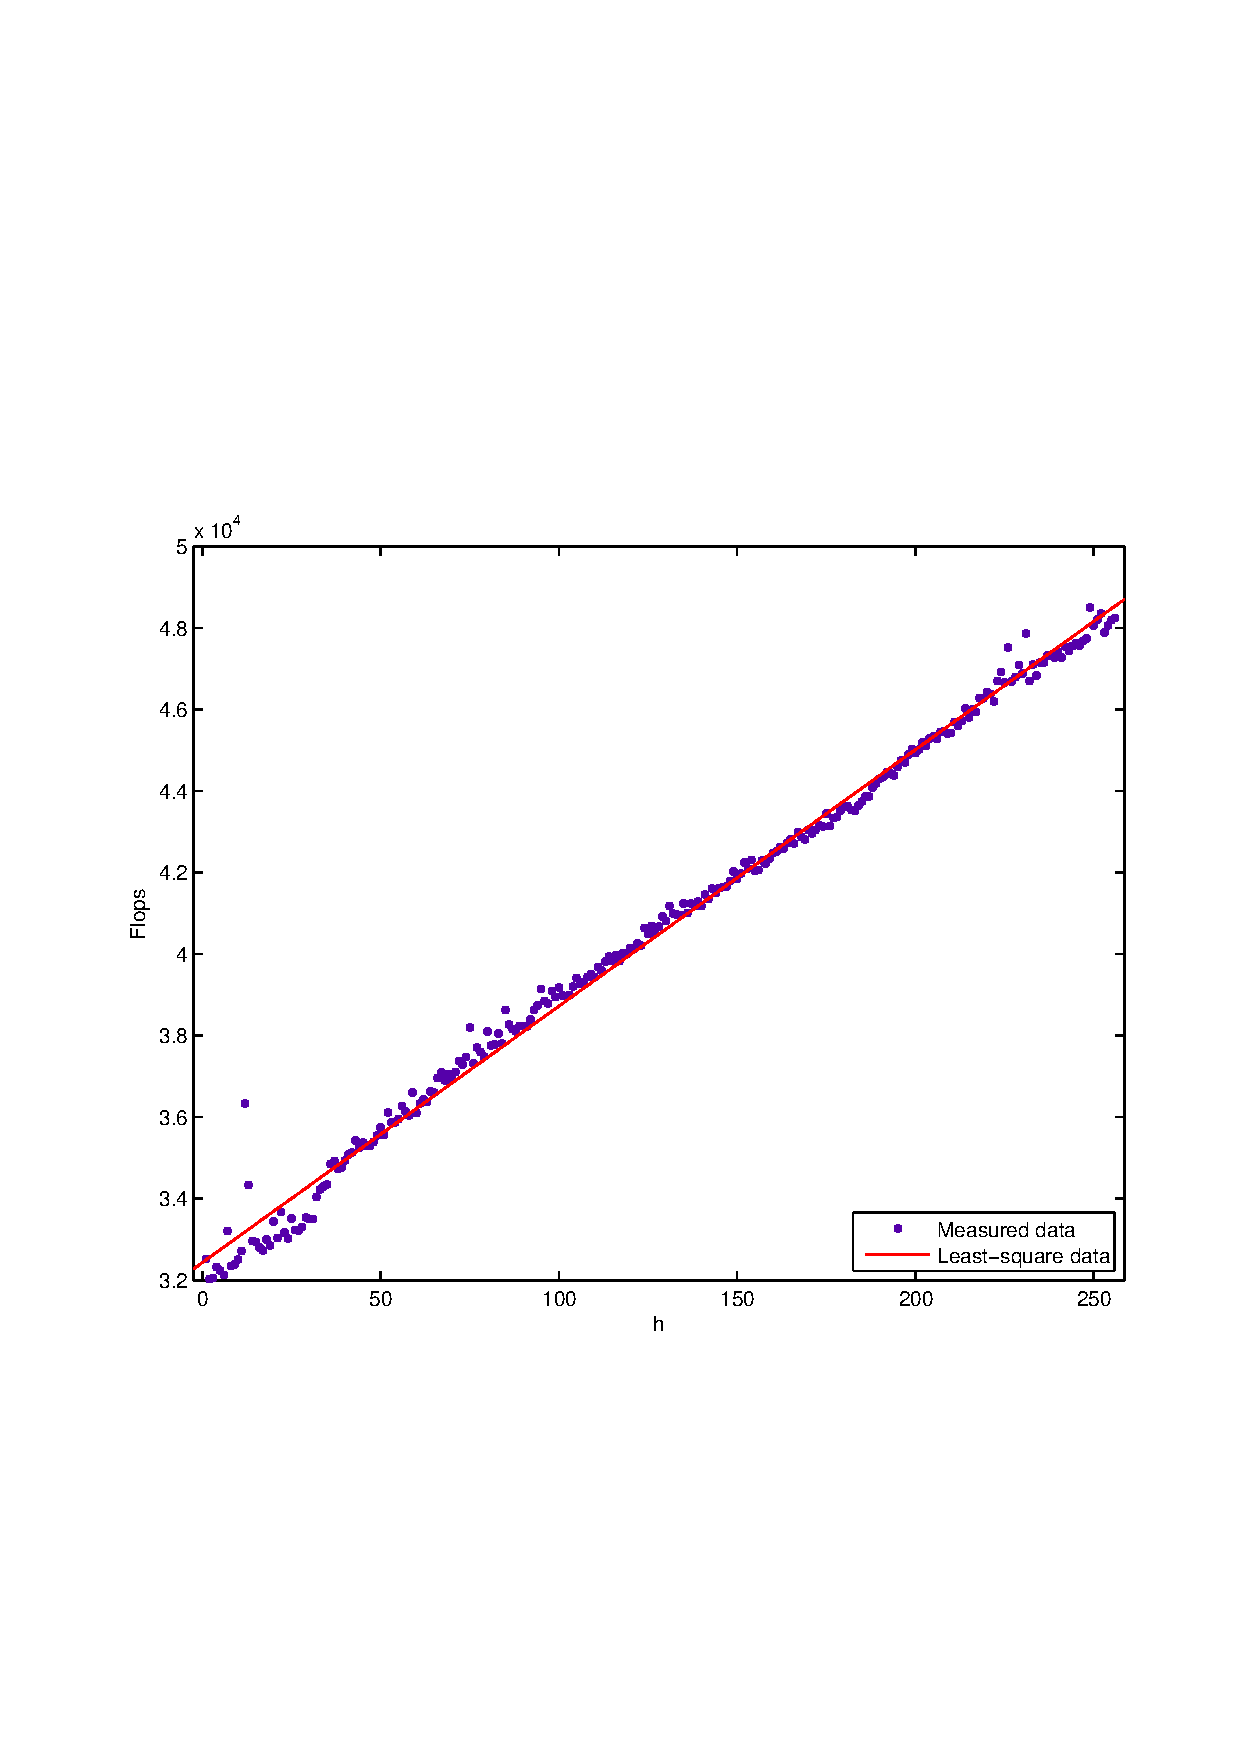
\includegraphics[scale=0.6]{img/32-put}
\end{center}
\caption{Huygens: $p=32$}\label{huy:32}
\end{figure}

\begin{figure}[H]
\begin{center}
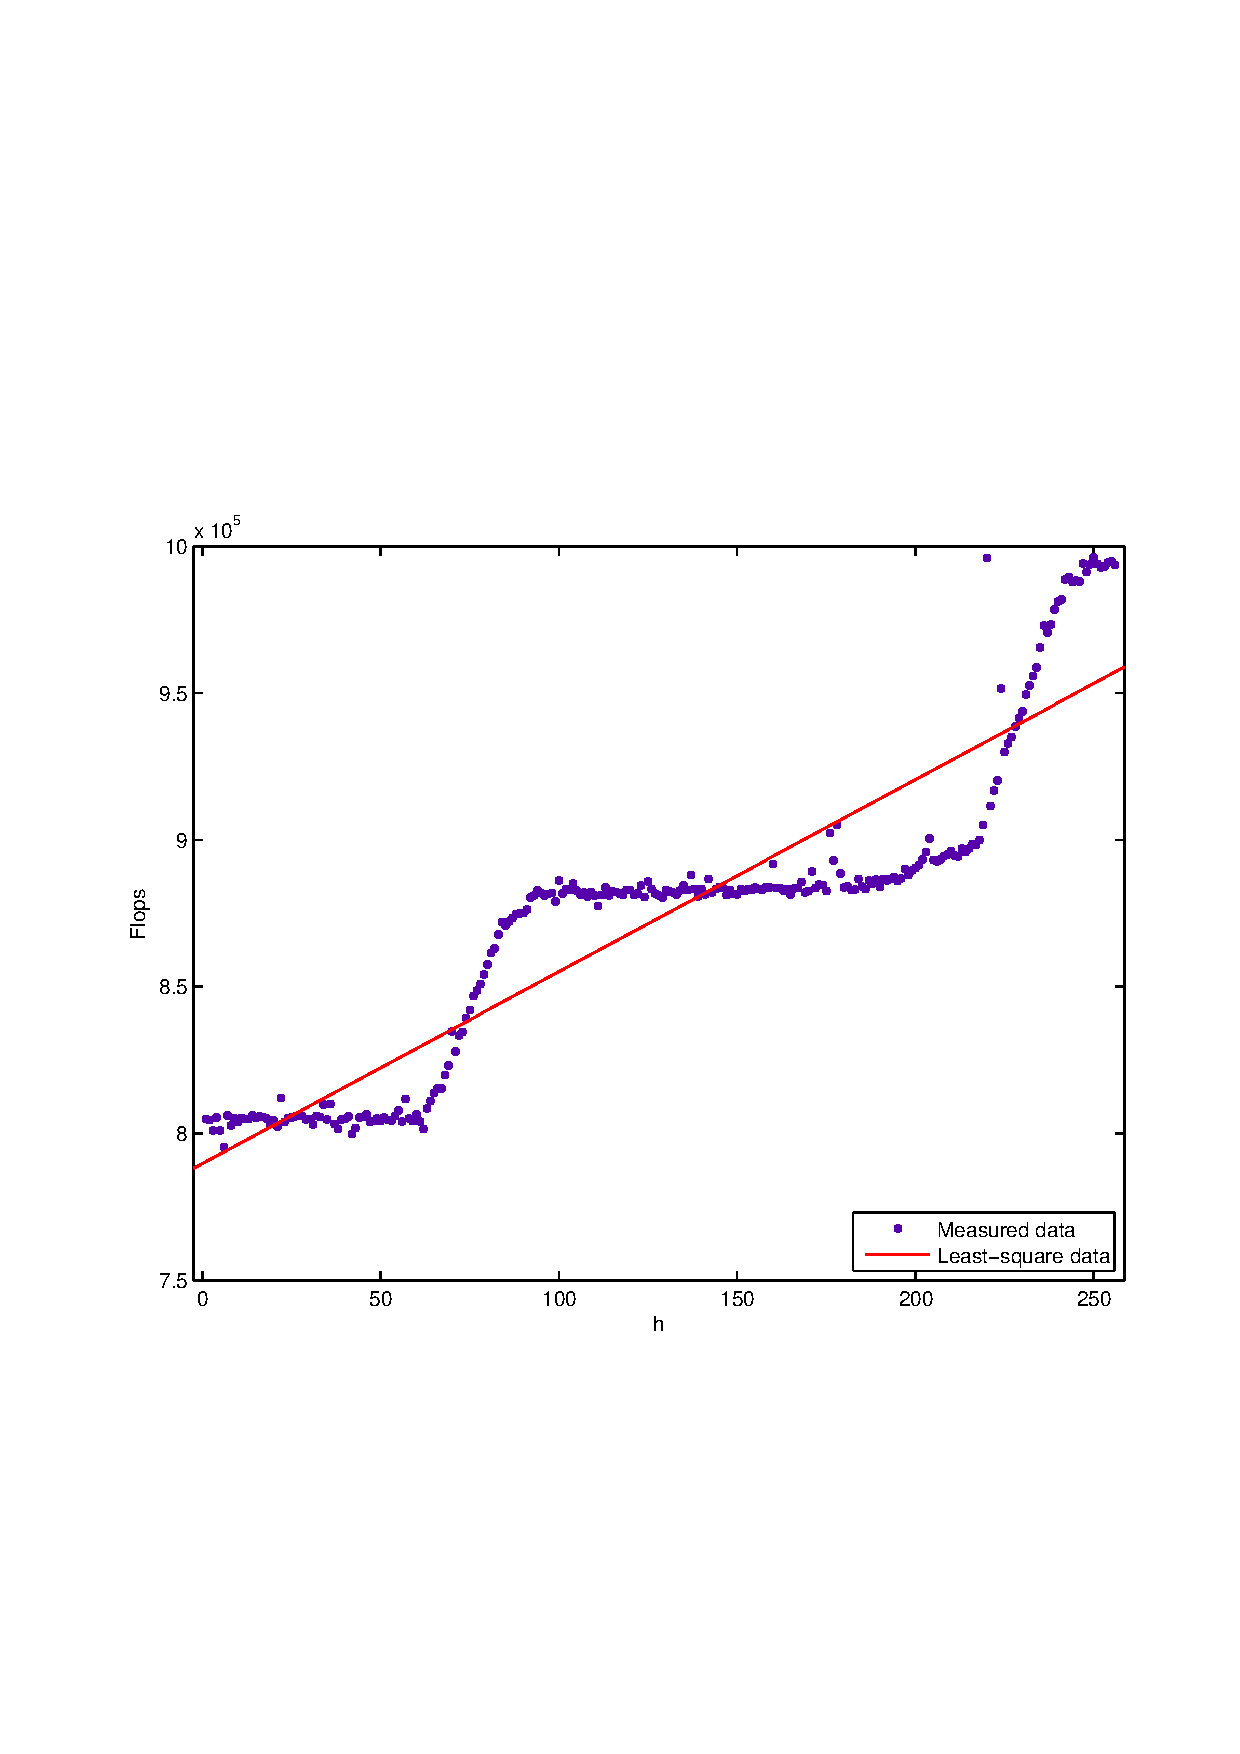
\includegraphics[scale=0.6]{img/abyssos-32-put}
\end{center}
\caption{Abyssos: $p=32$} \label{aby:32}
\end{figure}

\begin{figure}[H]
\begin{center}
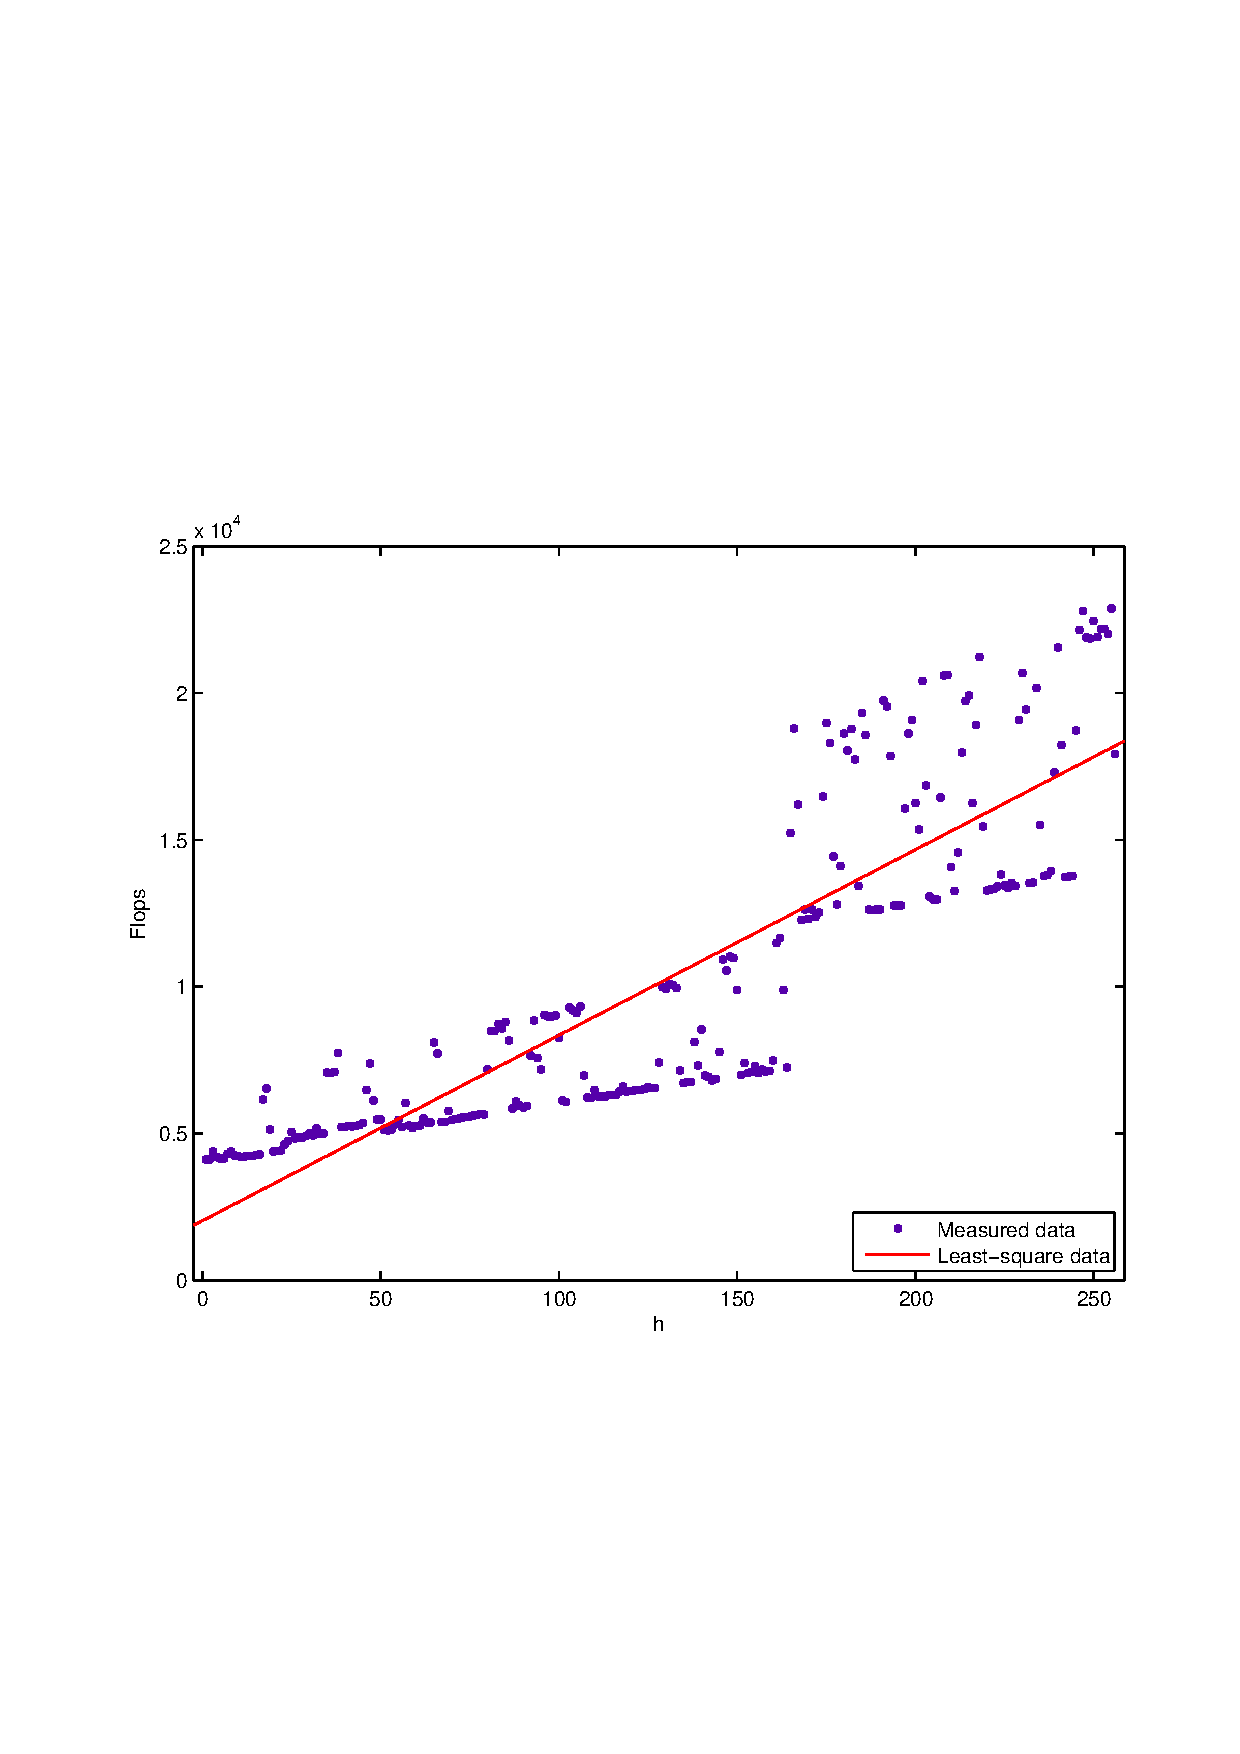
\includegraphics[scale=0.6]{img/mbair-2-put}
\end{center}
\caption{MacBook Air: $p=2$} \label{mbair:2}
\end{figure}

\begin{figure}[H]
\begin{center}
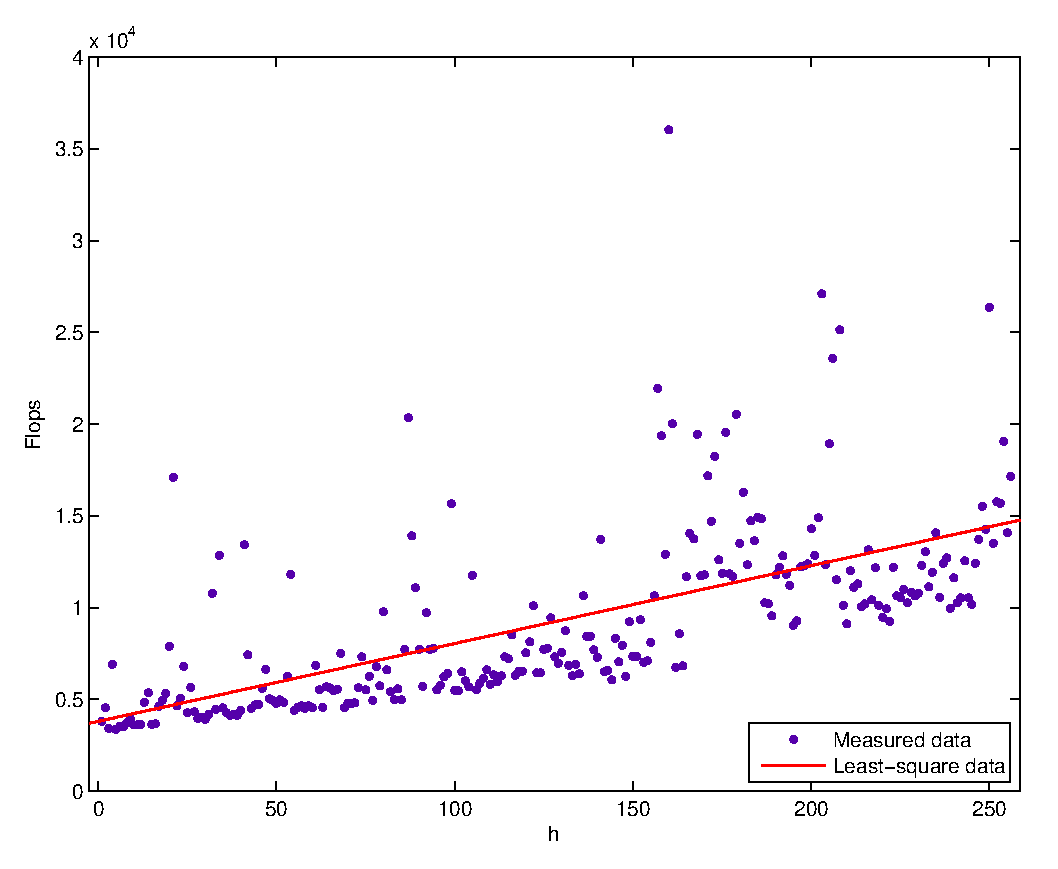
\includegraphics[scale=0.6]{img/mbpro-2-put}
\end{center}
\caption{MacBook Pro: $p=2$} \label{mbpro:2}
\end{figure}

\subsubsection{\texttt{bsp\_get}}

We also measured, for both the supercomputers, the performances when we replace \verb|bsp_put| by \verb|bsp_get|. The result are shown in Figures \ref{huy:32g} and \ref{aby:32g}:

\begin{figure}[H]
\begin{center}
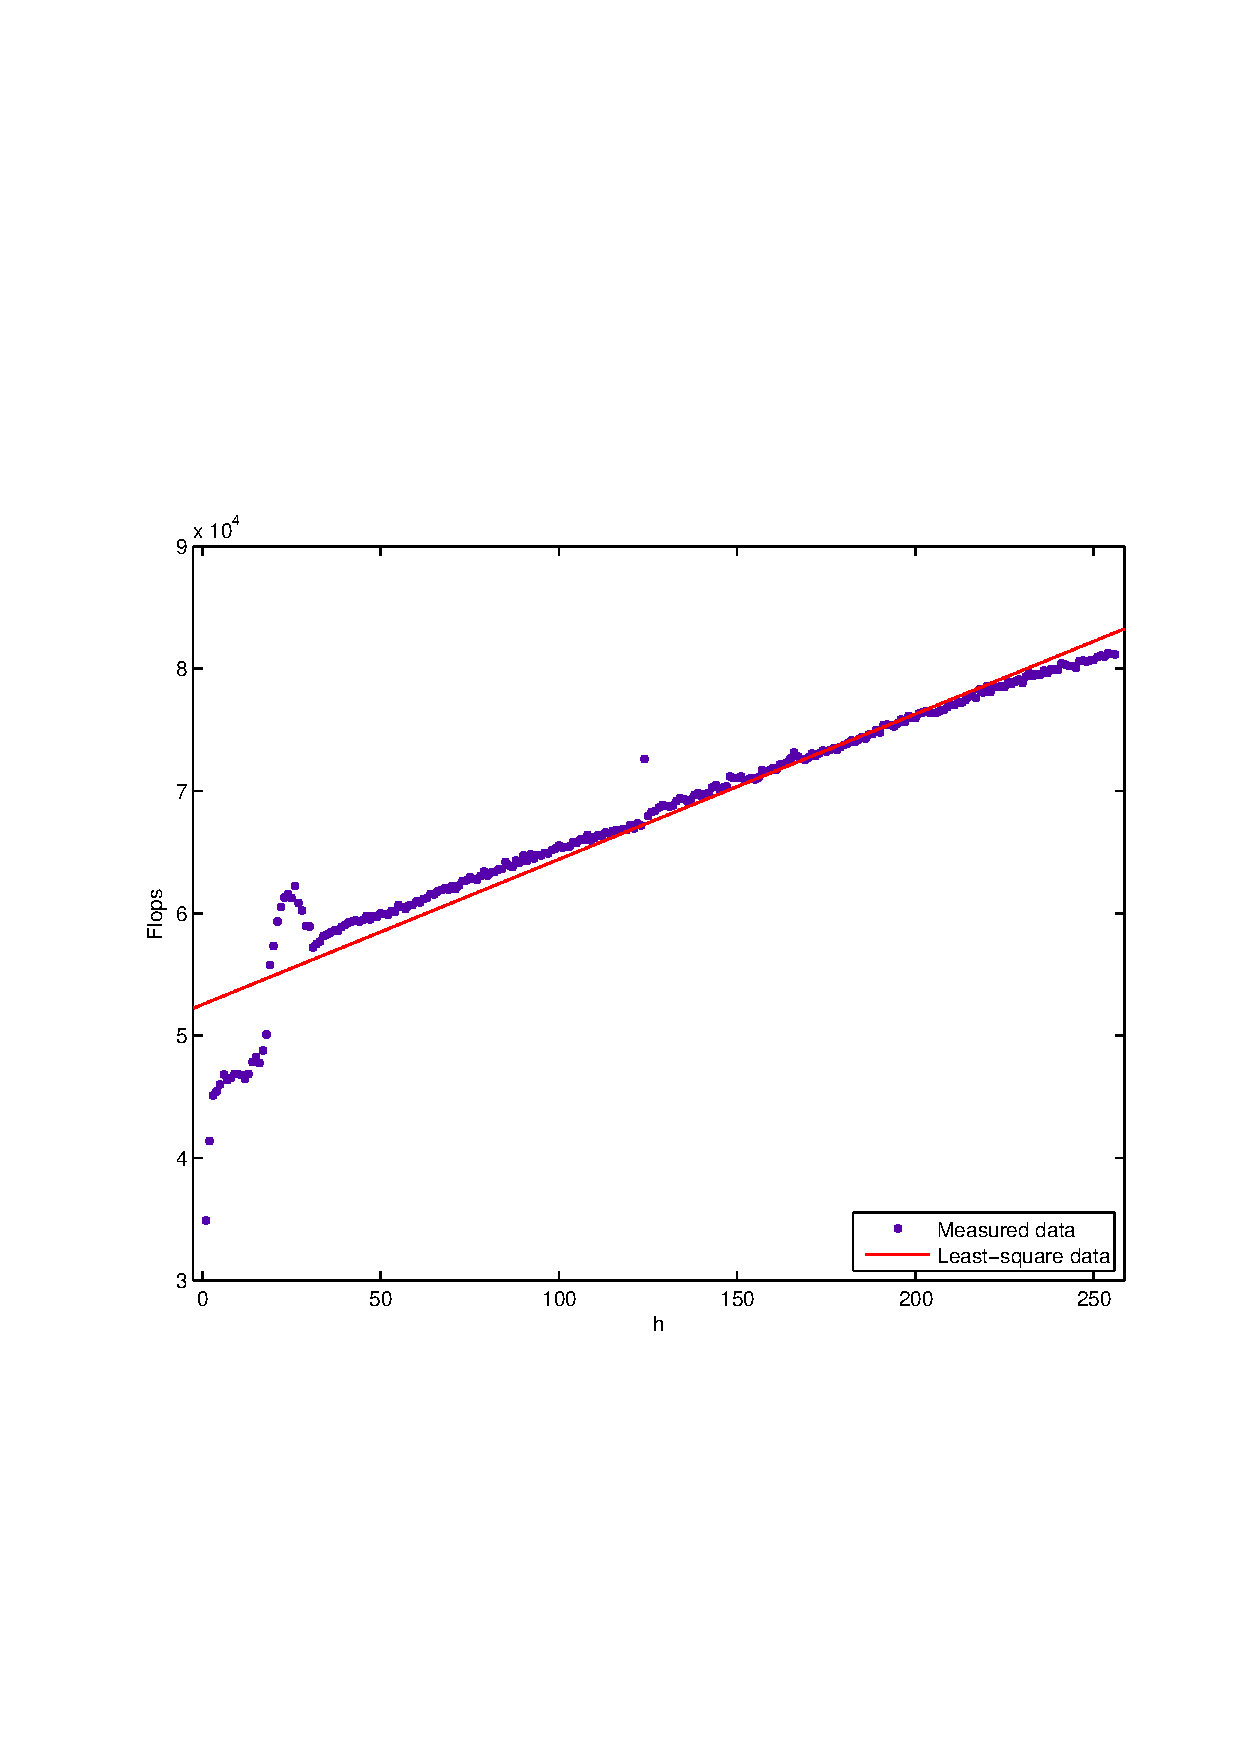
\includegraphics[scale=0.6]{img/32-get}
\end{center}
\caption{Huygens: \texttt{bsp\_get} and $p=32$} \label{huy:32g}
\end{figure}


\begin{figure}[H]
\begin{center}
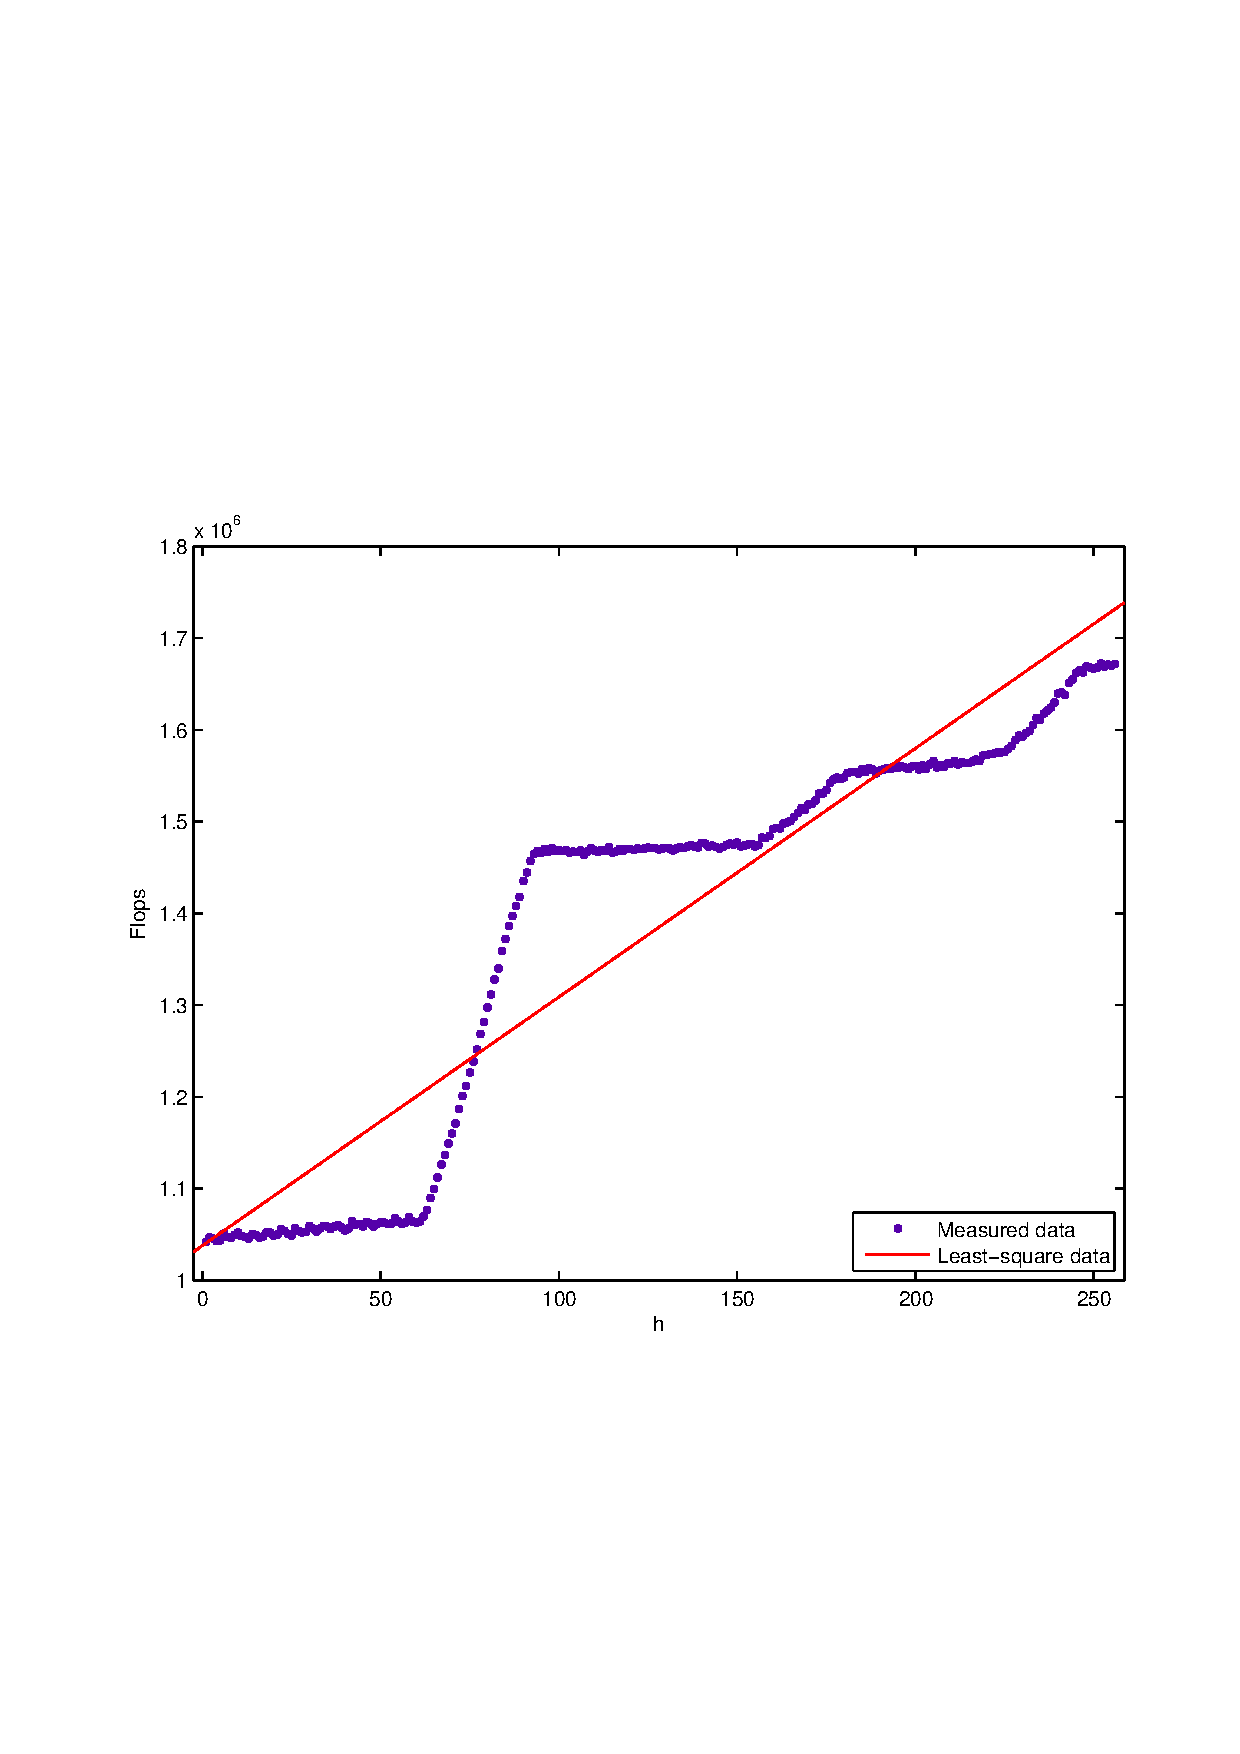
\includegraphics[scale=0.6]{img/abyssos-32-get}
\end{center}
\caption{Abyssos: \texttt{bsp\_get} and $p=32$} \label{aby:32g}
\end{figure}

\subsubsection{Remarks}

On Figure \ref{huy:32} we can see almost a linear increase of the Time (in flop units) with the increase of $h$. This is due to the fact that there was we reserved (and used) a full node of 32 cores on Huygens, thus elimintating any source of noise. If we change \verb|bsp_put| into \verb|bsp_get|, thus obtaining Figure \ref{huy:32g}, we can see a similar linear behaviour, with the exception of low values of $h$.

Abyssos, instead, shows a somewhat erratic behaviour. While we were almost the only users of the machine (so there should not be much noise from other running tasks) Figures \ref{aby:32} and \ref{aby:32g} show that, with respect to the increase of $h$, the behavior of the Time is descibed by altenrating phases of stagnation and phases rapid growth.

Figures \ref{mbair:2} and \ref{mbpro:2}, which we remember were obtained with $p=2$, then equal to number of physical cores, show that other running processes (from an Operating System, for example) interfere a lot with our benchmarks.

\subsection{Experimental results}

Since our implementation, from preliminary testing, seems reasonably fast, we run two series of tests: finding primes below $10^8$ and below $10^9$.

In the following tables we represent the machine, the number of processor used $p$, the time taken for the initial sequential step $t_{seq}$, the time taken to compute the result $t$ (we assume that each processor takes exactly the same time to compute the final result, but in reality there is a difference in timing at most of the order of $10^{-4} s$).

On the dutch supercomputer Huygens, we always reserved full nodes: 1 for $p=1,...,32$, 2 for $p=64$, and so on. For the sequential time we used the interactive mode, in order to take the time with \verb|time|; for this reason, it is important to remark that the result for the sequential algorithm may not be completely reliable since the processor used was also probably in charge of some other task, in the meantime. This is the reason we decided to run our parallel program even with $p=1$ and used this value for our Speedup plot (see below).

A similar thing also applies for the other supercomputer, Abyssos.

\subsubsection{Primes up to $10^8$}

With $N=10^8$, we have that $\sqrt{N} = 10000$. For the sequential time we used the UNIX function \verb|time|, while for the parallel program we used the function \verb|bsp_time|. The results are shown in Table \ref{tab:1e8}

\begin{table}
\begin{center}
\begin{threeparttable}
\begin{tabular}{|r r r|r r r|}
\hline
\multicolumn{3}{|c|}{Huygens} & \multicolumn{3}{c|}{Abyssos} \\
\hline
$p$ & $t_{seq}$ & $t$ & $p$ & $t_{seq}$ & $t$ \\
\hline
1 & & 3.195 & 1 & & 7.789 \\
1\tnote{1} &  0.000286  & 3.0742 & 1\tnote{1} & 0.000085 & 4.3123 \\
2 & 0.000296 & 1.5163 & 2 & 0.000061 & 2.1834 \\
4 & 0.000298 & 0.7253 & 4 & 0.000078 & 1.0743\\
8 & 0.000333 & 0.4309 & 8 & 0.000117 & 0.8701 \\
16 & 0.000380 & 0.2295 & 16 & 0.000058 & 0.3609 \\
32 & 0.000518 & 0.1553 & 32 & 0.000063 & 0.1000\\
64 & 0.000874 & 0.1235 & 64 & 0.000058 & 0.0752\\
128 & 0.000295 & 0.1114 & 112 & 0.000053 & 0.4309\\
256 & 0.000301 & 0.1258 & & &\\
\hline
\multicolumn{3}{|c|}{MacBook Air} & \multicolumn{3}{c|}{MacBook Pro} \\
\hline
1\tnote{1} & 0.000178 & 1.4846 & 1\tnote{1} & 0.000115 & 1.8095 \\
2 & 0.000137 & 1.0819 & 2 & 0.000151 & 1.3450 \\
4 & 0.000241 & 0.9434 & 4& 0.000192 & 1.1931 \\
\hline
\end{tabular}
\begin{tablenotes}
\item [1] \small{This is obtained running the parallel implementation with $p=1$, instead of the sequential algorithm.}
\end{tablenotes}
\end{threeparttable}
\caption{Results with $n=10^8$.} \label{tab:1e8}
\end{center}
\end{table}

In Figures \ref{sp1e8}-\ref{sp1e8m} we show the speedup plot for $p=1,...,32$ (with $p>32$ we noticed that the speedup plot is very noisy: it is hard to understand the real impact of the increased number of processors) for the supercomputers and for $p=1,..,4$ for the laptops.

\begin{figure}[H]
\begin{center}
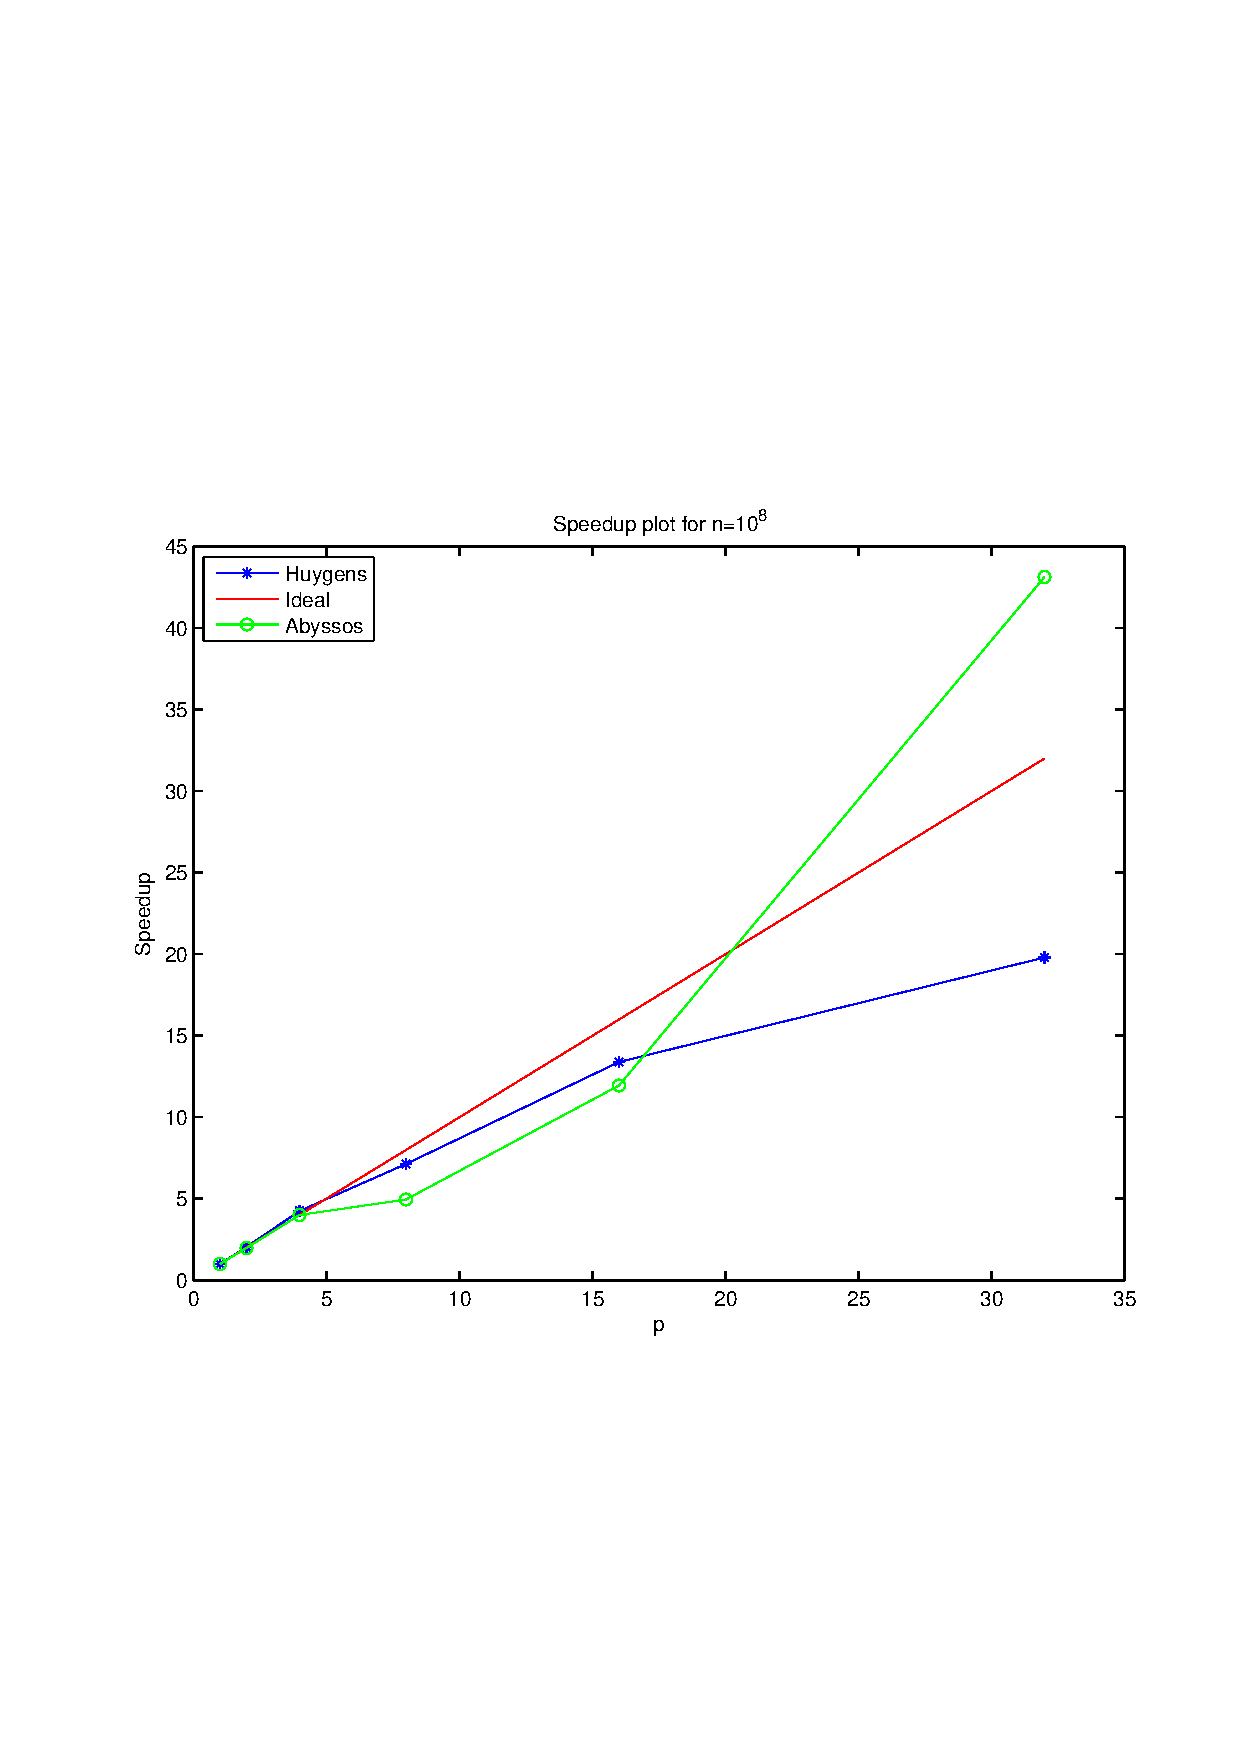
\includegraphics[scale=0.6]{img/sp1e8}
\end{center}
\caption{The speedup plots of the supercomputers, with $n=10^8$.} \label{sp1e8}
\end{figure}

\begin{figure}[H]
\begin{center}
\includegraphics[scale=0.6]{img/sp1e8m}
\end{center}
\caption{The speedup plots of the laptops, with $n=10^8$.} \label{sp1e8m}
\end{figure}


\subsubsection{Primes up to $10^9$}

If $n=10^9$, we have that $\sqrt{n} \simeq 31622$. In Table \ref{tab:1e9} we show the results.

\begin{table}[H]
\begin{center}
\begin{threeparttable}
\begin{tabular}{|r r r|r r r|}
\hline
\multicolumn{3}{|c|}{Huygens} & \multicolumn{3}{c|}{Abyssos} \\
\hline
$p$ & $t_{seq}$ & $t$ & $p$ & $t_{seq}$ & $t$ \\
\hline
1 & & 35.803 & 1 & & 29.383 \\
1\tnote{1} & 0.000845  & 35.6322 &  1\tnote{1} & 0.000145 & 48.7383  \\
2 & 0.000849 & 17.3429 & 2 & 0.000147 & 24.3291 \\
4 & 0.000864 & 8.6553 & 4 & 0.000151 & 21.1777 \\
8 & 0.000862 & 5.7959 & 8 & 0.000170 &  10.4823\\
16 & 0.000991 & 3.2012 & 16 & 0.000150 & 5.4085\\
32 & 0.001019 & 1.9018 & 32 & 0.000145 & 2.8799\\
64 & 0.000851 & 1.2257 & 64 & 0.000152 & 1.6304\\
128 & 0.000871  & 0.9219 & 112 & 0.000270 & 2.7395\\
256 & 0.000956 & 0.8252 & & & \\
\hline
\multicolumn{3}{|c|}{MacBook Air} & \multicolumn{3}{c|}{MacBook Pro} \\
\hline
1\tnote{1} & 0.000326 & 24.1877 & 1\tnote{1} & 0.000391  & 23.1023\\
2 & 0.000380 & 12.4197 &  2 &  0.000465 & 16.3168 \\
4 & 0.000515 & 11.8628 & 4 &  0.000481 & 13.8871 \\
\hline
\end{tabular}
\begin{tablenotes}
\item [1] \small{This is obtained running the parallel implementation with $p=1$, instead of the sequential algorithm.}
\end{tablenotes}
\end{threeparttable}
\caption{Results with $n=10^9$.} \label{tab:1e9}
\end{center}
\end{table}

In Figures \ref{sp1e9}-\ref{sp1e9m} we show the speedup plot with $p=1,...,32$ (not for $p>32$ for the same reasons as above) for Huygens and Abyssos and with $p=1,...,4$ for the laptops:

\begin{figure}[H]
\begin{center}
\includegraphics[scale=0.6]{img/sp1e9}
\end{center}
\caption{The speedup plots of the supercomputers, with $n=10^9$.} \label{sp1e9}
\end{figure}

\begin{figure}[H]
\begin{center}
\includegraphics[scale=0.6]{img/sp1e9m}
\end{center}
\caption{The speedup plots of the laptops, with $n=10^9$.} \label{sp1e9m}
\end{figure}

\section{Conclusions and further developments}

From the previous results, it is evident that a parallel approach for the generation of prime numbers using Erathostenes' Sieve is convenient: beside from the eventual noise due to concurrency with other users, we have been able to speed up considerably (think about $n=10^9$ and the difference between $p=1$ and $p=256$, passing from 35 seconds to less than one second) the generation of such numbers.

Interestingly, there exists a number of distributed project (which aim to imitate the behaviour of a parallel architecture, splitting the work into ``chunks'' and distributing them among people all over the world which volunteer their computers) which involve prime numbers (they do not use Erathostenes' Sieve like we did):

\begin{itemize}
\item GIMPS (Great Internet Mersenne Prime Search)\citep{gimps}: aims to search \emph{Mersenne prime numbers} (that is a prime number of the form $2^k-1$ with $k \in \N$). As of 08/11/2011, GIMPS has a sustained throughput of approximately 70 Tflops/s\citep{gimps2}
\item PrimeGrid\citep{primegrid}, which in reality is a collection of smaller projects (Cullen Prime Search, solving of the Prime Sierpinski Problem, Twin Prime Search, and so on)
\end{itemize}

\printbibliography
\end{document} 
